\section{Features}
In the following section the features of the DualSense controller will be explained.

\subsection{Overview}
\begin{itemize}
	\item \textbf{Connectivity} The DualSense controller can be used via Bluetooth or USB (USB C).
	\item \textbf{Integrated battery} Featuring an integrated battery the DualSense controller is best used via Bluetooth. The controller can be charged via USB type-C.
\end{itemize}

\begin{figure}[H]
    \centering
    \subfloat[\centering Front View]{{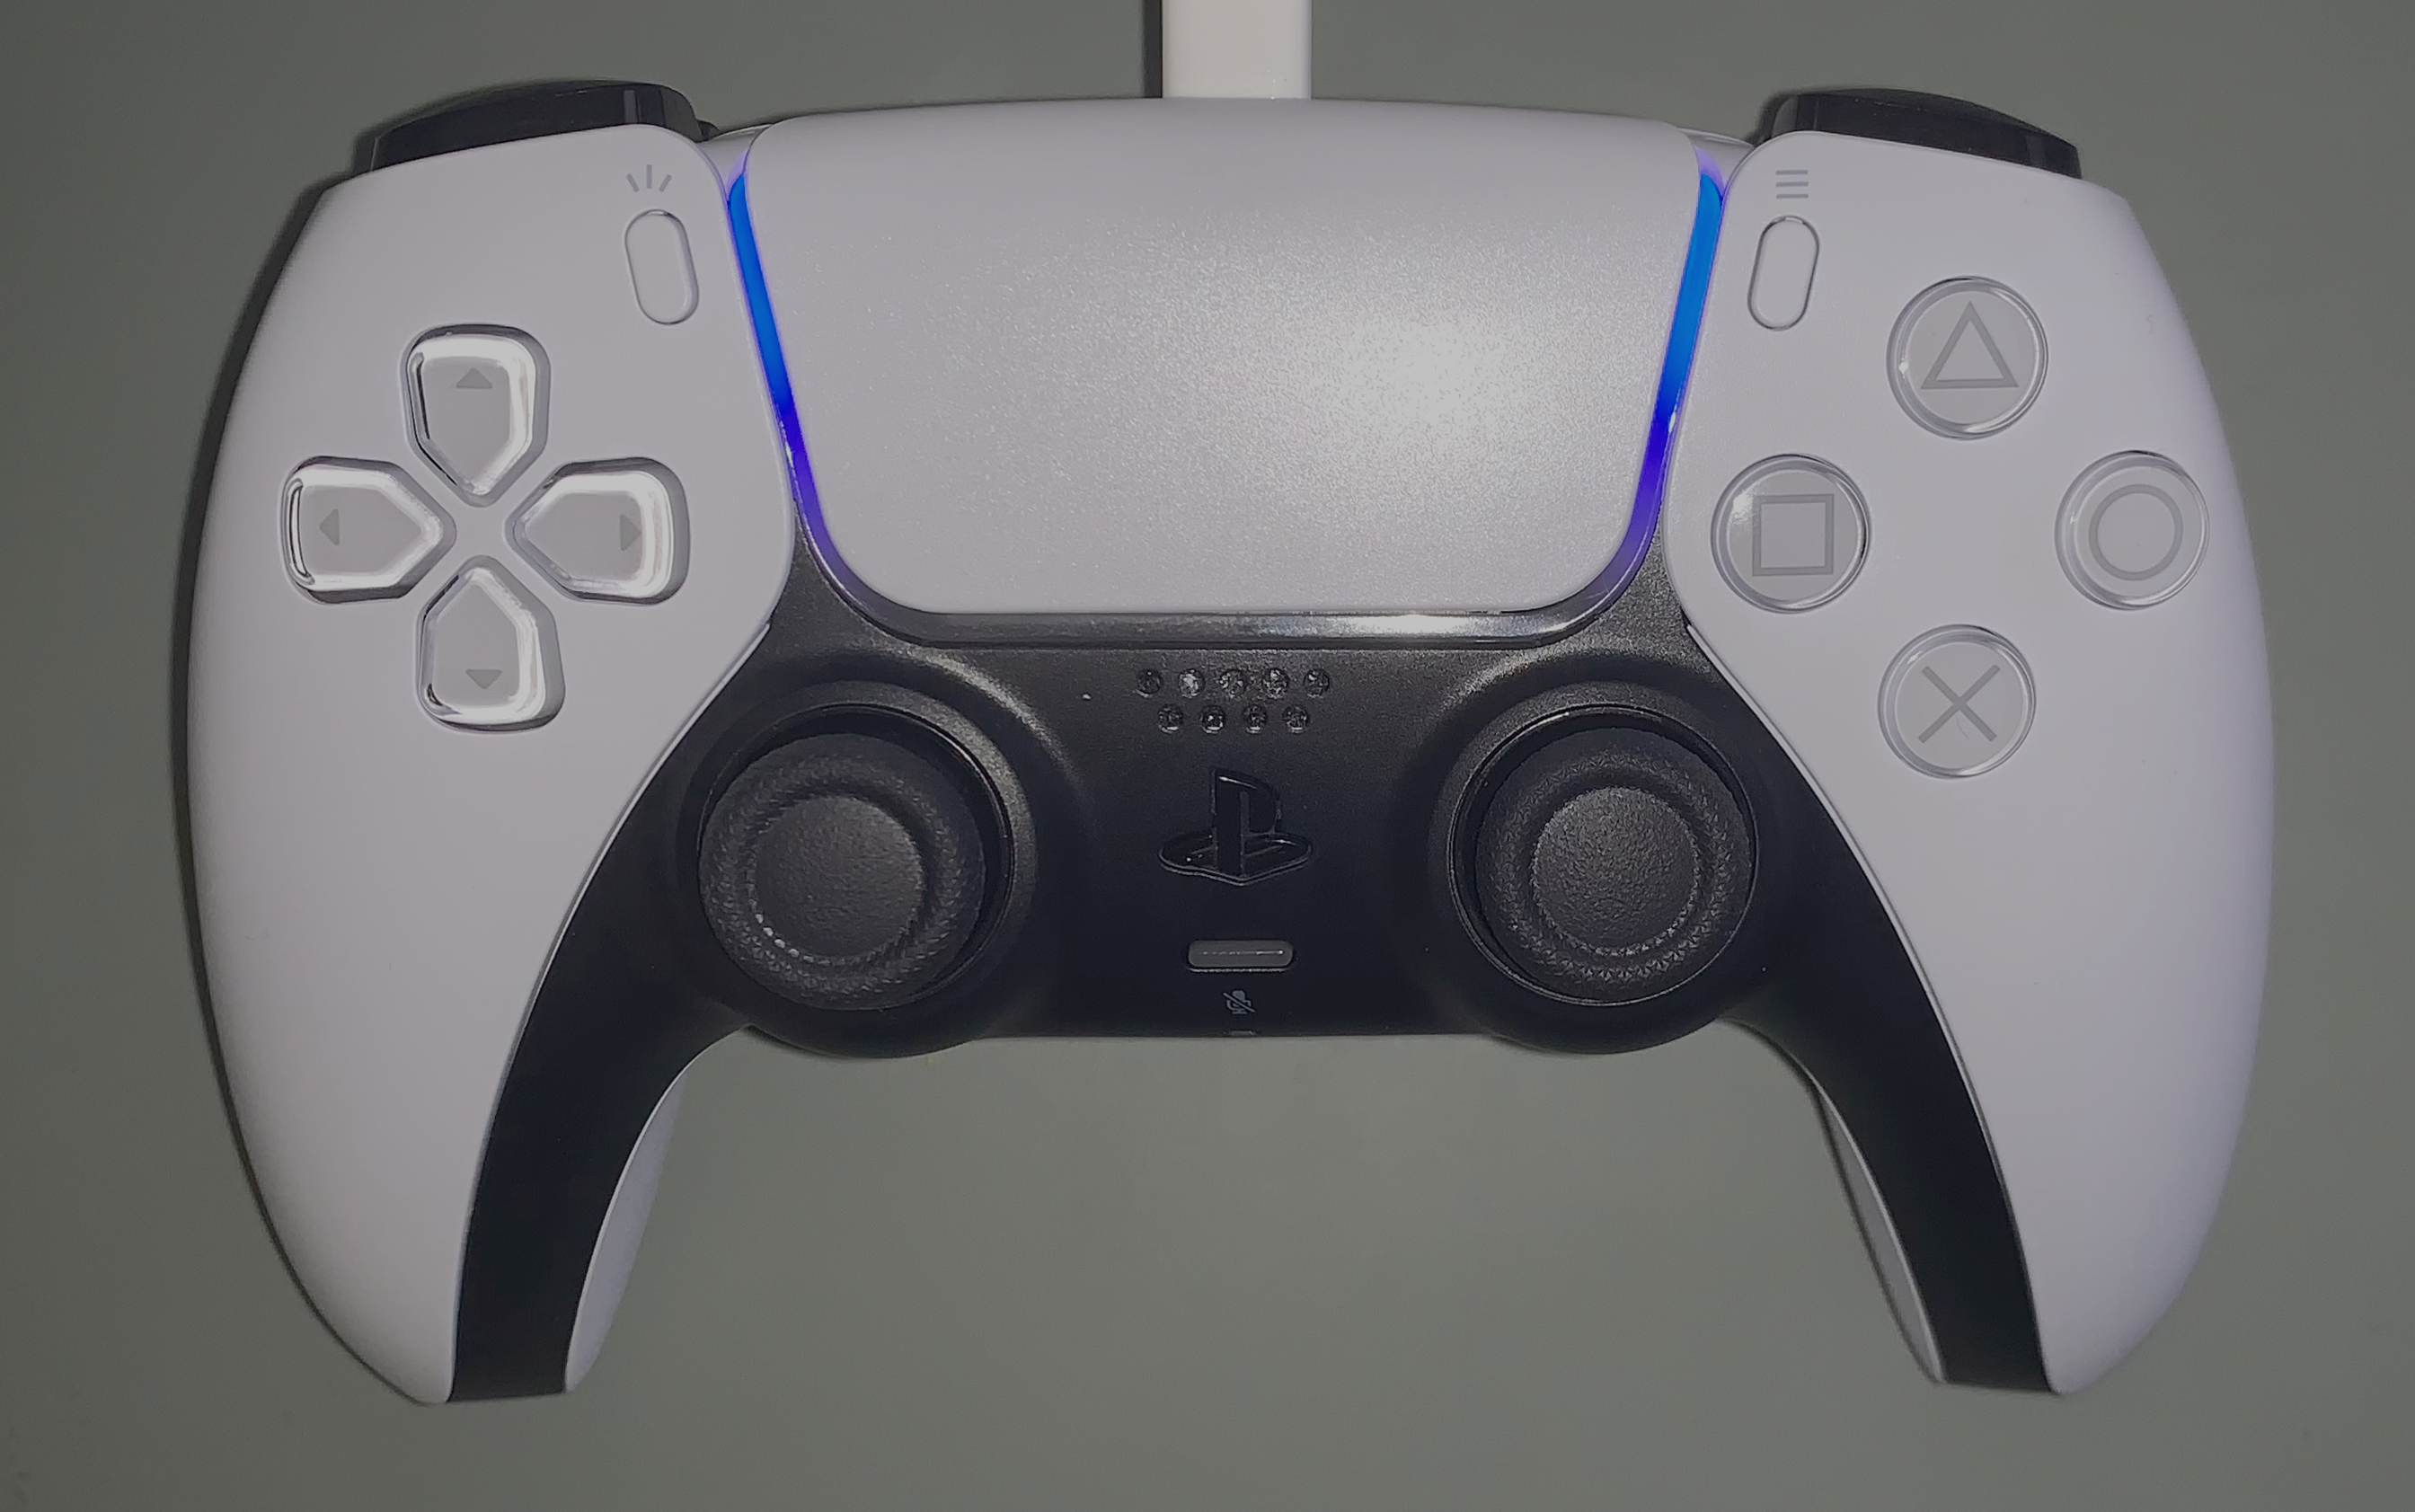
\includegraphics[width=5cm]{frontView} }}
    \qquad
    \subfloat[\centering Rear View]{{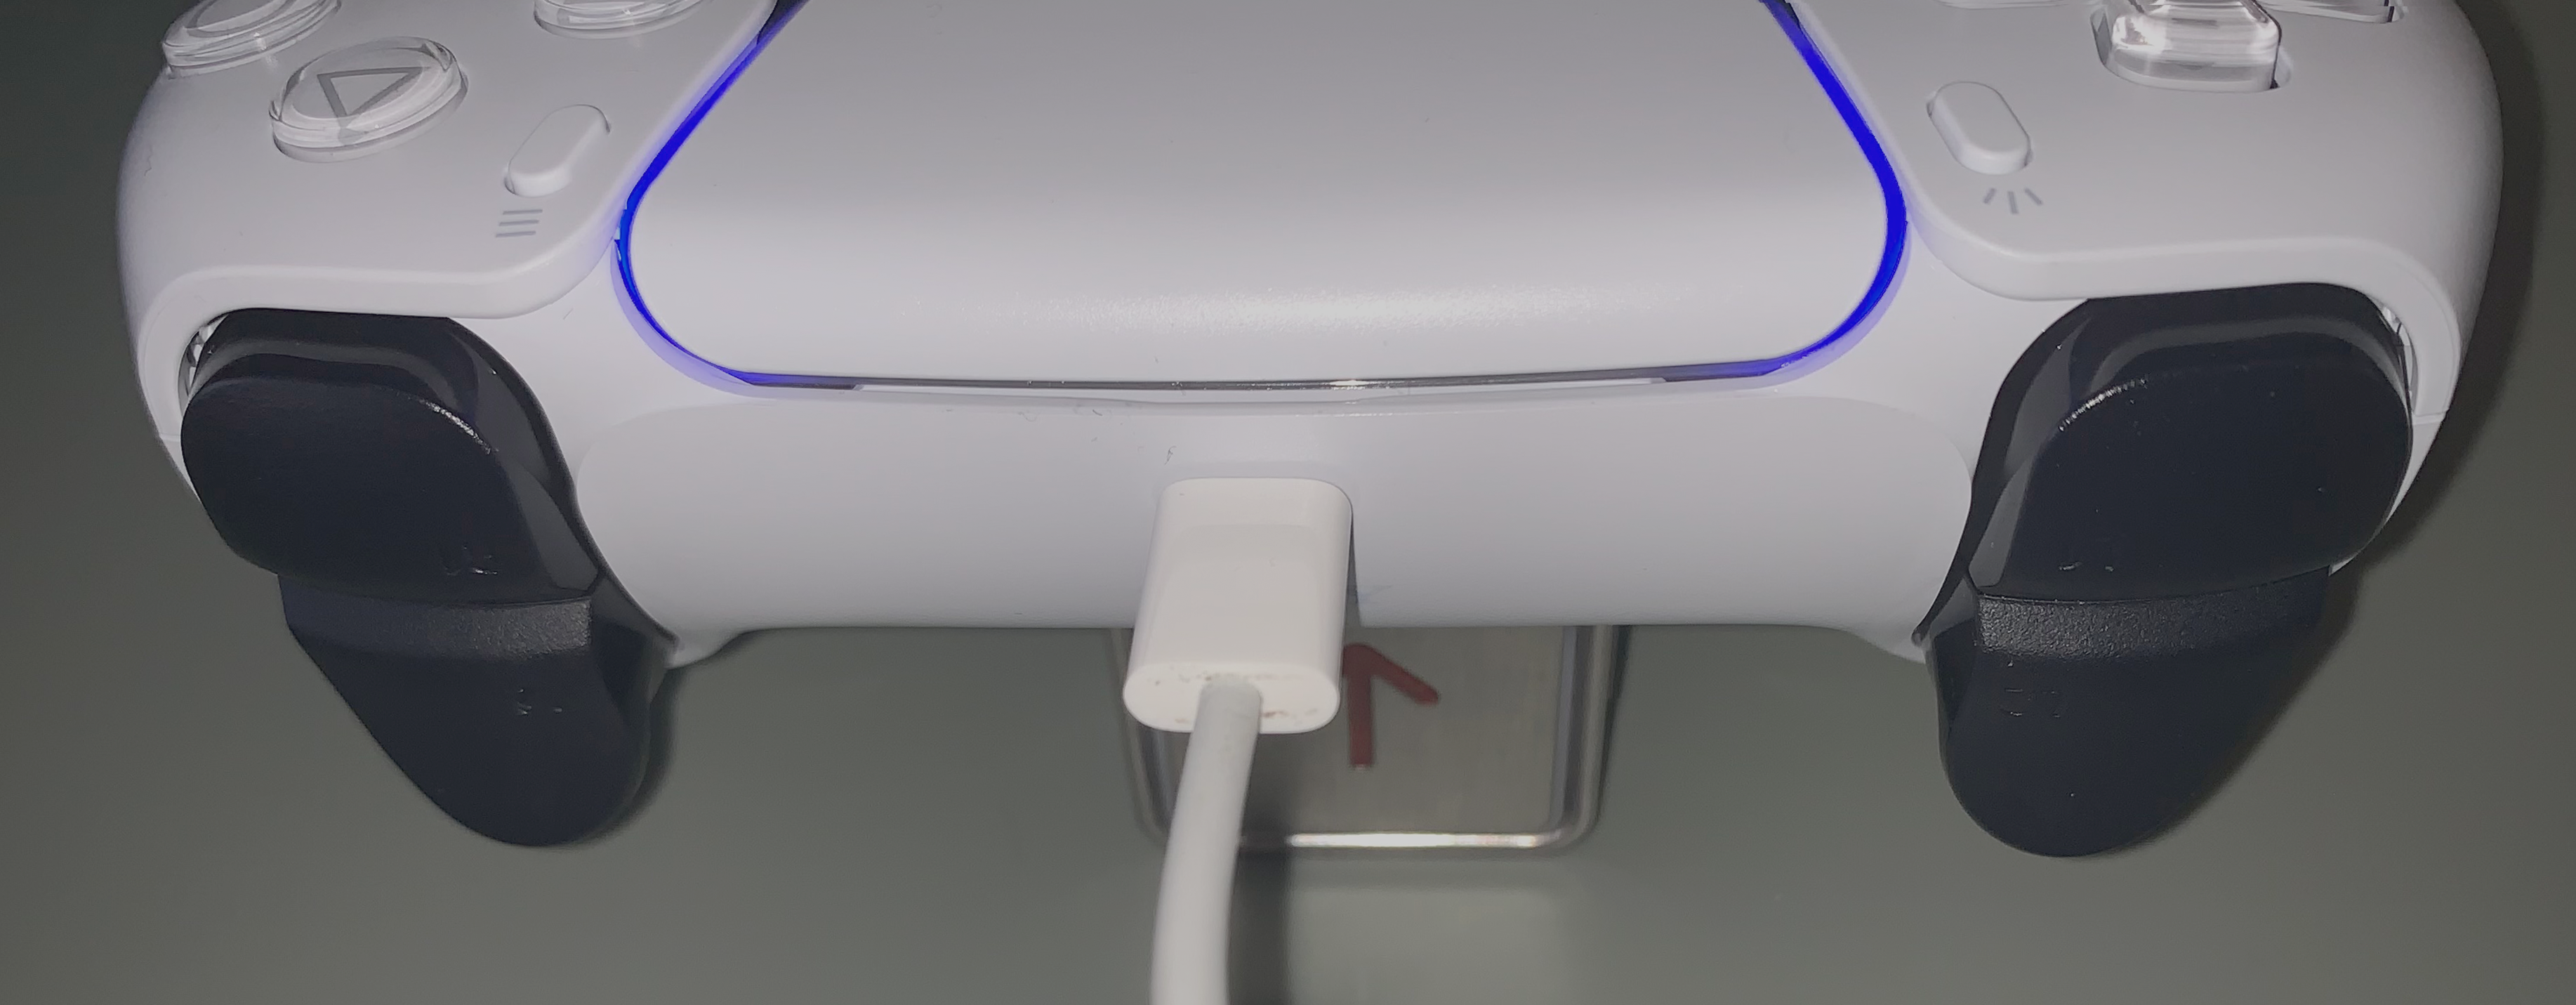
\includegraphics[width=5cm]{rearView} }}
    \caption{The DualSense controller}
\end{figure}

The DualSense controller features the following peripherals:
\begin{itemize}
	\item Two XY-Axis analog sticks with integrated push button.
	\item Two adaptive triggers (are able to provide feedback).
	\item Two shoulder buttons.
	\item DPad with the ability to press two neighbor buttons simultaneously.
	\item The default Square, Cross, Circle and Triangle PlayStation buttons.
	\item Dual-touch touchpad with integrated push button, surrounded with five player indication LEDs on the bottom and RGB-LED lightbar on the sides.
	\item Menu, share, microphone mute and PlayStation button.
	\item 3-Axis Accelerometer and Gyroscope.
	\item Two rumble motors (Hard and Soft one). Can alternatively used as haptic feedback (not supported yet).
	\item Integrated speaker and microphone.
	\item Stereo audio jack.	
\end{itemize}

\subsection{Feature List}

\paragraph{Analog sticks}
Each analog stick has two axis with 8-Bit precision each. The analog sticks will automatically return to their center position if released. They are mapped to the range $-128$ to $127$ where $0$ means center, $-128$ means left/bottom on X/Y-Axis and $127$ means right/top on X/Y-Axis. Using the analog values requires the correction of the dead zones, because a released stick will most likely not have the value $R_{xy}(0; 0)$ it will be a bit off. Same goes for the extreme values witch will also be off and not be exactly $T_{xy}(0; 127)$, $L_{xy}(-128; 0)$, etc..
\begin{figure}[H]
    \centering
    \subfloat{{\includegraphics[width=8cm]{frontView_sticks} }}
    \caption{Analog sticks}
\end{figure}

\paragraph{Adaptive trigger}
The DualSense controller feature two 8-Bit analog triggers. It is possible to read the trigger values as 8-Bit continuous values or alternatively as binary button input. Aside of the normal trigger operation the adaptive triggers can be configured to simulate various force feedback effects. It is possible for example to simulate a gun trigger.
\begin{figure}[H]
    \centering
    \subfloat{{\includegraphics[width=8cm]{rearView_trigger} }}
    \caption{Adaptive triggers}
\end{figure}

\paragraph{Bumpers}
The two L/R Bumpers located over the adaptive triggers can be read as normal button inputs.
\begin{figure}[H]
    \centering
    \subfloat{{\includegraphics[width=8cm]{rearView_bumpers} }}
    \caption{L/R Bumpers}
\end{figure}

\paragraph{DPAD and PS Buttons}
The DualSense controller feature a DPAD and the default well know PlayStation Square, Cross, Circle and Triangle buttons. The DPAD is capable of registering two simultaneously pressed buttons, however the two buttons must be neighbors. The PS-Buttons are being registered as four individual binary values.
\begin{figure}[H]
    \centering
    \subfloat{{\includegraphics[width=8cm]{frontView_mainbtn} }}
    \caption{DPAD and PS-Buttons}
\end{figure}

\paragraph{Other Buttons}
The DualSense controller feature several more buttons. Thees are:
\begin{itemize}
	\item \textbf{Menu button} Should be used to open the in-game menu.
	\item \textbf{Share button} Should be used to open the in-game photo mode.
	\item \textbf{PlayStation button} Can be used to open a in-game overlay (Look at the know issues to get an additional use case of this button).
	\item \textbf{Mic button} Should be used to mute the microphone.
\end{itemize}
All the listed buttons are readable through individual binary values.
\begin{figure}[H]
    \centering
    \subfloat{{\includegraphics[width=8cm]{frontView_other} }}
    \caption{Left to right, top to bottom: Share, Menu, PlayStation and Mic Button}
\end{figure}

